\chapter{Web applicatie}\label{ch:implementatie}

In dit hoofdstuk leggen we uit hoe de verschillende concepten zijn ge\"implementeerd. We beschrijven de gebruikte berekeningen, simulaties en overwegingen.

\section{Architectuur}

Er zijn veel mogelijkheden voor het maken van een app. Talen zoals Python, C++, Java, ... kunnen gebruikt worden om een app te ontwikkelen die lokaal uitgevoerd kan worden. Daarnaast kunnen ook JavaScript, HTML en CSS, met eventueel frameworks, worden ingezet om een webapp te maken.

Omdat we een zo toegankelijk mogelijke app willen bieden, hebben we besloten om een webapp te ontwikkelen. Hierdoor kan de app door iedereen gebruikt worden zonder dat er een installatie nodig is. 

% We willen echter niet dat de app onbruikbaar wordt wanneer deze niet online is, daarom moet de app ook offline beschikbaar zijn.
% % SUBJECT TO CHANGE

% Om dit te realiseren wordt op de github pagina van de app een gids voorzien om de app
% lokaal uit te voeren. Daarnaast wordt de mogelijkheid voorzien om de app ook makkelijk via de flask backend lokaal te hosten.

\subsection{Frontend}

De webapp is geschreven in Vue.js, een Javascript-framework dat werkt met componenten en reactiviteit biedt. Deze reactiviteit zorgt ervoor dat de gebruiker direct de effecten van gemaakte aanpassingen kan zien. Andere vergelijkbare opties zijn React en Angular, maar we kozen voor Vue.js omdat het de effici\"entste van de drie is voor het maken van kleine, maar toch performante apps.  

Voor de vele gebruikte standaardcomponenten (zoals knoppen, inputs, ...) maken we gebruik van het Vuetify Vue-componentframework.

We besloten om de frontend in twee talen aan te bieden: Nederlands en Engels. Dit wordt ge\"implementeerd met I18n ~\cite{krukowskiVue3I18n2023}. Via JSON-bestanden wordt voor elke taal de tekst die in de webapp gebruikt moet worden bijgehouden. De gebruiker kan eenvoudig veranderen van taal aan de hand van een knop in de app.

\subsection{Backend}

Het grootste deel van de berekeningen wordt in de webapp zelf uitgevoerd en dus op het apparaat van de client. Dit minimaliseert het aantal calls naar de server en de daarbijhorende laadtijden. We minimaliseren het aantal calls omdat we het belangrijk vinden dat de gebruiker het effect van zijn aanpassingen zo snel mogelijk ziet. Dit omdat we de gebruiker willen kunnen laten spelend leren. Als de gebruiker dan telkens vrij lang moet wachten op resultaten is dit niet mogelijk. Toch worden enkele complexere berekeningen naar de backend verplaatst. Dit komt omdat Javascript niet de meest geschikte taal is voor deze berekeningen en omdat dergelijke berekeningen het apparaat van de gebruiker te veel kunnen belasten. Toch proberen we er bij deze berekeningen ook voor te zorgen dat de tijd tot het krijgen van resultaten zo minimaal mogelijk is.

Om de complexe berekeningen uit te voeren maken we gebruik van een Python-backend met Flask. We kiezen voor Python vanwege de vele libraries voor datamanipulatie en wiskundige berekeningen, zoals numpy en scipy. Bovendien bestaat er een Python-library genaamd luxpy~\cite{smetTutorialLuxPyPython2020}, die veel berekeningen voor licht en kleur al implementeert. Deze library wordt onder andere gebruikt voor het berekenen van de \gls{cri} en Ra-waardes, het genereren van een tm30-rapport en de berekeningen voor hyperspectral image rendering.

Omdat we willen dat de reactie van de backend zo rap mogelijk is maken we gebruik van websockets. Alternatief zouden we gebruik kunnen maken van HTPP, maar dit is niet even effici\"ent. We kiezen echter voor websockets vanwege hun lagere latency.

\section{Algemene structuur}

We hebben de webapp opgedeeld in drie onderdelen. Ten eerste is er een onderdeel voor de inputs. Ten tweede is er een onderdeel voor de verschillende outputs. Ten slotte is er een onderdeel waarin de gebruiker de gebruikte modellen kan bekijken en aanpassen. We zorgen ervoor dat de inputs altijd zichtbaar zijn voor de gebruiker, omdat dit essentieel is. We willen namelijk dat de gebruiker altijd met de inputs kan spelen om te leren. Het is minder belangrijk dat alle verschillende outputs altijd zichtbaar zijn. Daarom hebben we ervoor gekozen om voor elk type output een tablad te voorzien. Daarnaast voorzien we een laatste tablad voor het databeheer. Hier kan de gebruiker de gebruikte modellen bekijken en aanpassen.

\subsection{Inputs}

In het inputgedeelte past de gebruiker verschillende componenten aan met behulp van input fields en sliders, en ziet de effecten hiervan in het outputgedeelte. De gebruiker kan kiezen uit drie standaardtypes inputs: \gls{led}s, fosforen en quantum dots. De gebruiker kan zes van deze componenten selecteren, bijvoorbeeld drie \gls{led}s, twee fosforen en \'e\'en quantum dot. We kozen ervoor zes inputs aan te bieden omdat dit voldoende speelruimte laat, maar ook realistisch blijft.

\subsection{Outputs}

De output is opgesplits in zes verschillende tabladen.

\begin{itemize}
    \item SPD
    \item Chromaticiteit
    \item Color rendering
    \item ''realistic rendering''
    \item led visualisatie
    \item databeheer
\end{itemize}

In het SPD-venster bekijkt de gebruiker de spectra van \gls{led}s via een grafiek. Daarnaast ziet de gebruiker hoe verschillende luminescente materialen deze spectra be\"invloeden. Dit venster dient als initieel inzicht in de gemaakte \gls{led}.

In het chromaticiteitsvenster bekijkt de gebruiker de chromaticiteit van de \gls{led}s en eventuele luminescente materialen. Dit biedt inzicht in de kleur van de \gls{led}s en de invloed van luminescente materialen op die kleur. Dit is cruciaal voor het leren over het ontwerpen van witte \gls{led}s. Dit venster dient voor de gebruiker als een eerste inzicht in de kleur van de gemaakte \gls{led}.

In het color-renderingvenster ziet de gebruiker de color rendering metrieken (\gls{cri} of tm30) van de \gls{led}s en luminescente materialen. Hierdoor krijgt de gebruiker een beter beeld van hoe goed de \gls{led}s kleuren kunnen weergeven, wat essentieel is voor de perceptie van de belichting. Dit venster dient dus voor de gebruiker als een inzicht in de kleurweergave van de gemaakte \gls{led}.

In het ''realistic rendering''-venster krijgt de gebruiker een realistische weergave van de verlichting in een ruimte. De app toont hierbij standaard een vergelijking met D65 (daglicht) om een beter beeld te geven van hoe de verlichting er in werkelijkheid uit zou zien. Deze vergelijking kan ook aangepast worden naar een aantal andere belangrijke lichtbronnen. Dit venster dient dus voor de gebruiker om te leren over hoe de belichting met de gemaakte \gls{led} er in werkelijkheid uit zou zien.

In het led-visualisatievenster krijgt de gebruiker een idee van hoe de chip van de gemaakte \gls{led} eruitziet. De visualisatie toont \gls{led}s als gekleurde rechthoeken, fosforen als gekleurde kristallen en quantum dots als gekleurde puntjes. In dit venster kan de gebruiker op een eenvoudige manier leren over hoe een \gls{led} chip eruit zou kunnen zien. 

In het ''data management''-venster beheert de gebruiker de data van de app. Hier bekijkt de gebruiker welke modellen worden gebruikt voor de spectra van \gls{led}s en luminescente materialen. Daarnaast kan de gebruiker eigen luminescente materialen toevoegen, het referentiespectrum voor color rendering aanpassen en het type color rendering wijzigen. Tot slot biedt de app een methode om een eigen formule te gebruiken voor de standaard spectra van luminescente materialen en het model voor de \gls{led}s.

\section{Structuur Vue}

De webapp in Vue is opgebouwd met een structuur van componenten en views. De views vormen de verschillende pagina's van de app, terwijl de componenten de herbruikbare onderdelen zijn die binnen deze views gebruikt worden. We kozen ervoor slechts gebruik te maken van \"e\"en view om de app zo eenvoudig mogelijk te houden.

Het werken met componenten biedt als voordeel dat ze herbruikbaar zijn. Zo gebruiken we bijvoorbeeld binnen het databeheer tablad meerdere dezelfde componenten voor het tonen van modellen. Daarnaast kunnen componenten worden aangepast met ''properties''. Zo kan de gebruiker bijvoorbeeld zelf inputs defini\"eren, die vervolgens in de views worden toegepast.

De webapp bestaat uit een groot aantal componenten en \'e\'en view. Omdat de app uit veel componenten bestaat, moeten we deze onderling kunnen laten communiceren. Zo moeten we bijvoorbeeld de \gls{cct} waarde die in het ene component berekend wordt versturen naar een ander component. We kunnen dit bijvoorbeeld doen aan de hand van ''events'', waarbij een component een event stuurt dat door een andere component wordt opgevangen. 

Wanneer componenten die niet direct aan elkaar gekoppeld zijn data moeten delen, kan dit complex worden. Zo zou bijvoorbeeld als een component een event moet sturen naar een ver verbonden component een keten afgelegd moeten worden. Dit betekent dat \'e\'en component een event ontvangt en dit moet doorsturen. Dit gaat zo verder tot de bestemming. Om dit te vereenvoudigen, maken we in de app gebruik van ''pinia'' stores. Deze globale structuren slaan data op en maken deze beschikbaar voor componenten, waardoor het delen van data tussen verschillende componenten eenvoudig blijft. Daarnaast kunnen we in pinia stores gebruik maken van de ''persistent'' state om caching toe te voegen. Het is echter niet altijd beter om stores te gebruiken, omdat dit de app complex kan maken. Daarnaast zijn stores ook minder efficient.


\begin{figure}[H]
    \centering
    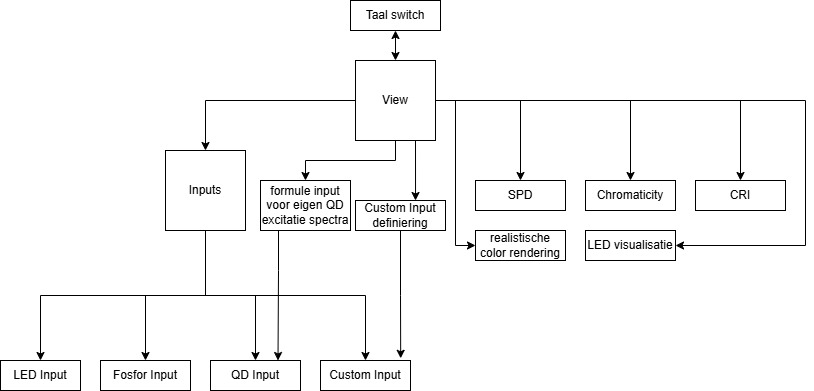
\includegraphics[width=0.9\linewidth]{structuur.jpg}
    \caption{Structuur Vue app}%
    \label{fig:vue_structure}
\end{figure}

\section{Implementatie inputs}

De inputs vormen het belangrijkste onderdeel van de app. Via deze inputs zorgen we ervoor dat de gebruiker kan experimenteren en leren van de effecten van zijn aanpassingen. De app biedt, zoals eerder vermeld, drie standaardtypes inputs: inputs voor \gls{led}s, fosforen en quantum dots.

Naast deze standaardinputs kan de gebruiker ook een input voor een luminescent materiaal maken met een csv-bestand en enkele scaling parameters. We bieden de mogelijkheid om eigen inputs te maken voor niet lerende gebruikers om te kunnen experimenteren. Zo kan bijvoorbeeld iemand die met een specifiek luminescent materiaal wil experimenteren dit doen. Deze input biedt echter wel minder flexibiliteit dan de standaardinputs, aangezien alleen de scaling parameters en de \gls{plqy}-waarde aangepast kunnen worden, dit omdat we bij deze input gebruik maken van vaste spectra en geen aanpasbare modellen.  

Voor het werken met de inputs kiest de gebruiker via een selectiemenu. Hierbij maken we gebruik van de reactiviteit van vue om enkel de geselecteerde inputs te tonen. We doen dit aan de hand van conditional rendering, waarbij alle componenten wel ingeladen zijn, maar enkel de geselecteerde effectief getoond worden.

We slaan de data van de inputs op in een van de eerder vermelde ''pinia'' stores. We maken gebruik van deze store omdat we de data van de inputs moeten gebruiken in verschillende componenten. Zo wordt bijvoorbeeld de data gebruikt om de stralingsstroom te berekenen, maar ook om de chromaticiteit te berekenen.

\subsection{LED Input}

Om een \gls{led} toe te voegen, moet de gebruiker een \gls{led} selecteren uit de beschikbare inputtypes. Vervolgens kan de gebruiker de parameters waarmee hij/zij wil experimenteren aanpassen met behulp van input fields en sliders. We kozen ervoor de fields en sliders te gebruiken omdat dit de gebruiker zowel toelaat specifieke waarden in te geven en met waarden te spelen.

We kozen ervoor om de \gls{led} input te beperken tot de belangrijkste parameters.

\begin{itemize}
    \item Centrale golflengte
    \item \gls{fwhm}
    \item Ingangsvermogen
    \item \gls{eqe}
\end{itemize}

We kozen voor deze parameters omdat deze de belangrijkste zijn voor het maken van een \gls{led}. De centrale golflengte en \gls{fwhm} bepalen de kleur van de \gls{led}, het ingangsvermogen bepaalt de lichtstroom en de \gls{eqe} bepaalt hoe effici\"ent de \gls{led} is in het omzetten van elektrische energie naar licht. Dit zijn dan ook de parameters die het belangrijkste zijn om al spelend te leren over de eigenschappen van \gls{led}s.

We kozen ervoor de \gls{eqe}-waarde onaanpasbaar te laten omdat deze waarde uit een model komt. De gebruiker kan echter wel de \gls{eqe}-waarde aanpassen door een eigen model te gebruiken (\cref{sec:eqe}).

\begin{figure}[H]
    \centering
    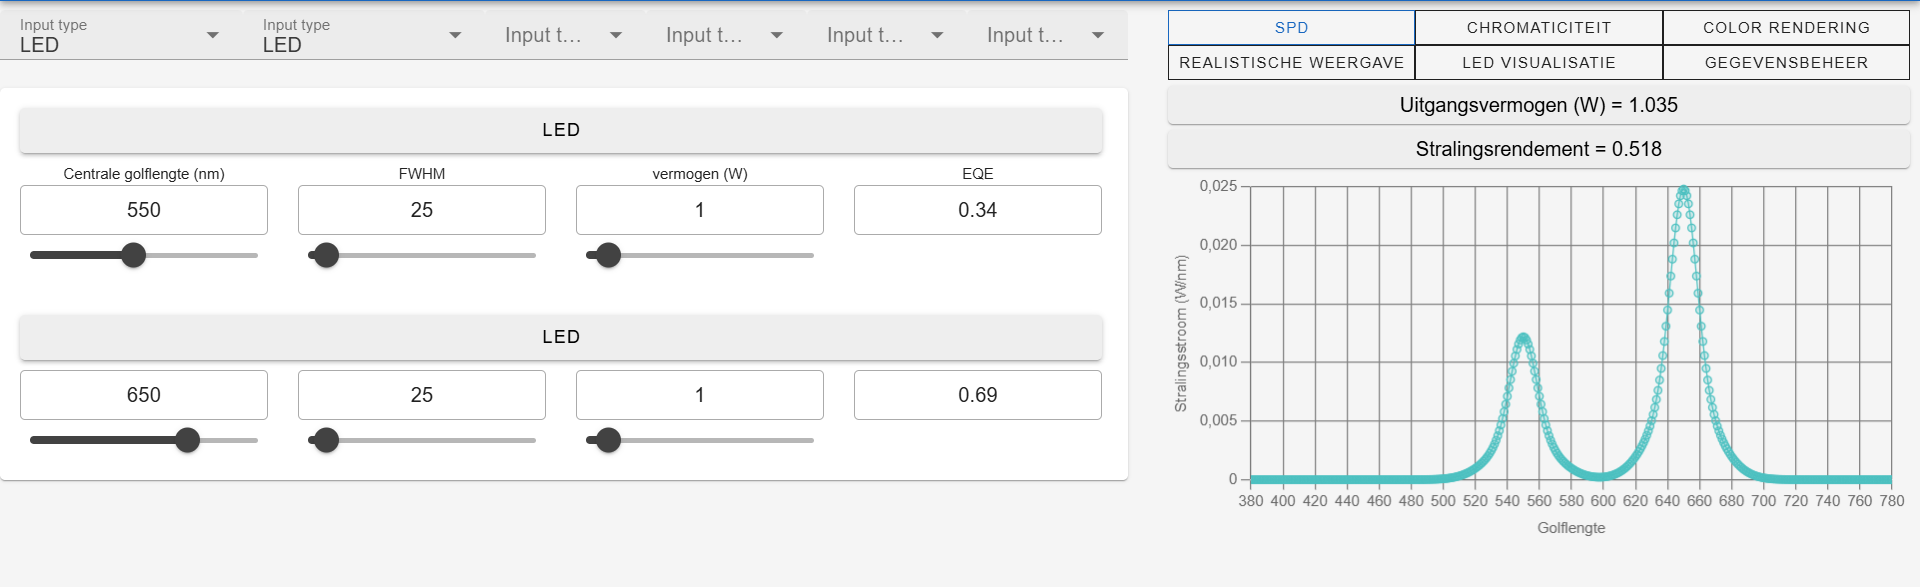
\includegraphics[width=1\linewidth]{figs/led_input.png}
    \caption{Voorbeeld \gls{led} inputs}%
    \label{fig:led_input}
\end{figure}

\subsection{Fosfor input}

Net zoals bij de \gls{led} input, moet de gebruiker voor het werken met fosforen een fosfor selecteren uit de beschikbare inputtypes. Hierbij voorzien we opnieuw input fields en sliders om de parameters specifiek en spelend aan te kunnen passen.

We kozen ervoor de volgende parameters aan de gebruiker aan te bieden.

\begin{itemize}
    \item Centrale excitatiegolflengte
    \item Centrale emissiegolflengte
    \item Excitatiebandbreedte
    \item Emissiebandbreedte
    \item concentratie
    \item \gls{plqy}
\end{itemize}

Deze parameters zijn de belangrijkste voor het maken van een fosfor. De centrale golflengtes en bandbreedtes bepalen de kleur van de fosfor, de concentratie bepaalt de hoeveelheid energie die de fosfor kan absorberen en de \gls{plqy} bepaalt hoe effici\"ent de fosfor is in het omzetten van geabsorbeerde energie naar licht. Daarnaast kan de gebruiker aan de hand van de centrale golflengtes leren over de gevolgen van de stokes shift (\cref{sec:witte-leds}).

We kozen ervoor om bij het selecteren van een fosfor de excitatiebandbreedte, emissiebandbreedte en \gls{plqy} standaardwaarden te geven.

\begin{itemize}
    \item Excitatiebandbreedte: 90 nm
    \item Emissiebandbreedte: 100 nm
    \item \gls{plqy}: 0.9
\end{itemize}

Deze waarden zijn standaardwaarden die een realistisch beeld geven van een gewoonlijk fosfor.

\begin{figure}[H]
    \centering
    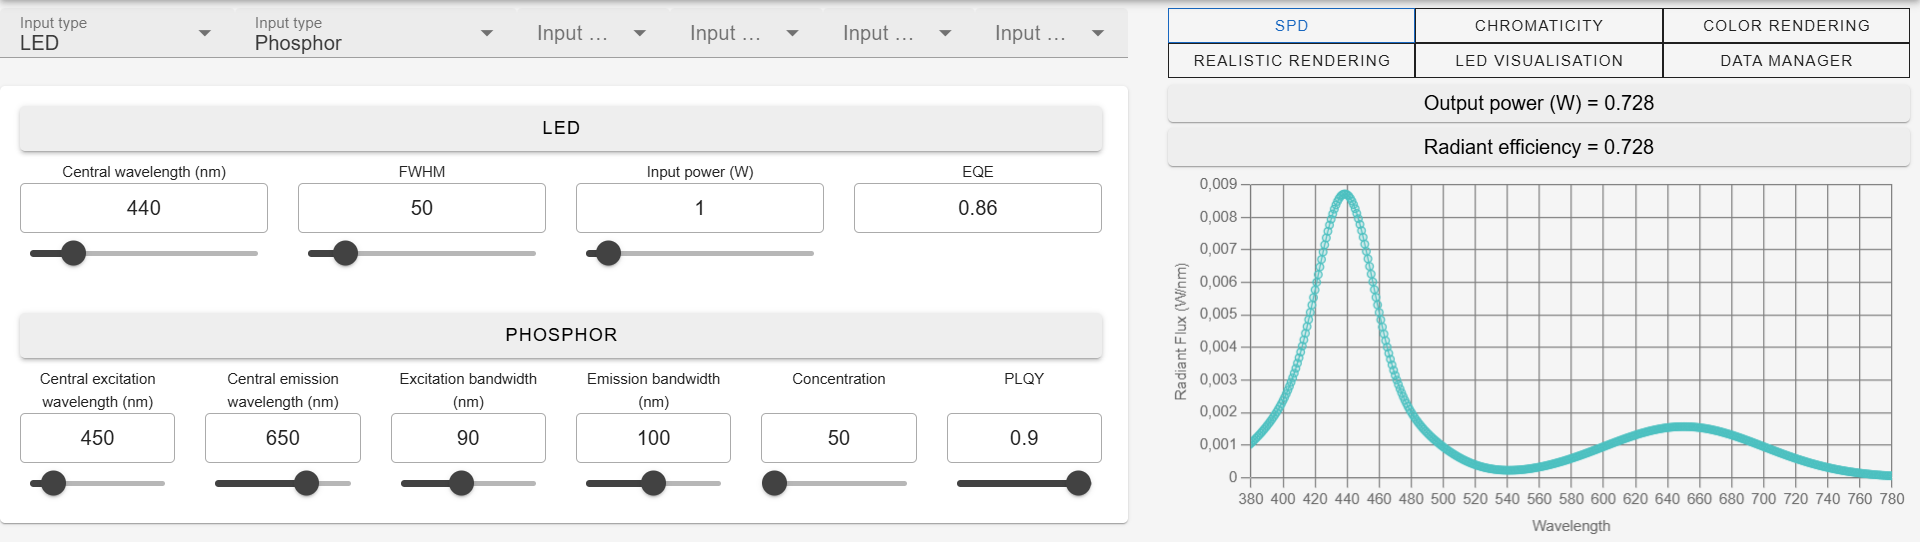
\includegraphics[width=1\linewidth]{fosfor_input.png}
    \caption{Voorbeeld fosfor inputs}%
    \label{fig:phos_input}
\end{figure}

\subsection{Quantum dot input}

De quantum dot input lijkt op de fosfor input. De gebruiker past, net zoals bij de fosfor input, de centrale emissiegolflengte, emissiebandbreedte, concentratie, en PLQY-waardes aan. De parameters voor de excitatie blijven echter onveranderd, omdat het standaardmodel voor het excitatiespectrum geen centrale excitatiegolflengte gebruikt. Wanneer echter een aangepaste formule wordt gebruikt, kan de gebruiker deze waarden wel aanpassen.

Voor de inputparameters die overeenkomen met de fosfor input gebruiken we achterliggend dezelfde variabelen. We doen dit op deze manier om zo het aantal parameters in de ''pinia'' stores zo gelimiteerd mogelijk te houden. Zo zorgen we ervoor dat de app zo effici\"ent mogelijk blijft.

Net zoals bij de fosfor input, voorzien we standaardwaarden voor de emissiebandbreedte en \gls{plqy}.

\begin{itemize}
    \item Emissiebandbreedte: 40 nm
    \item \gls{plqy}: 0.8
\end{itemize}

\begin{figure}[H]
    \centering
    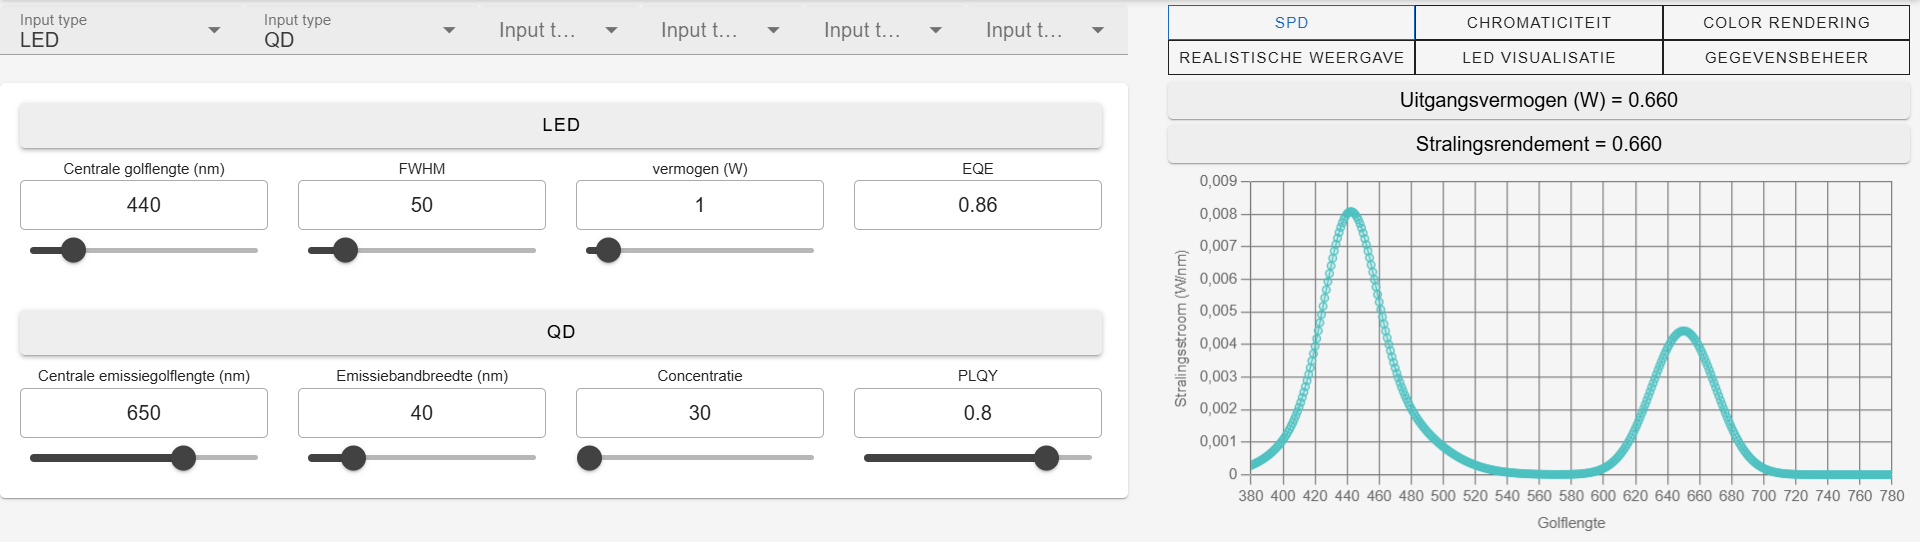
\includegraphics[width=1\linewidth]{QD_input.png}
    \caption{Voorbeeld quantum dot inputs}%
    \label{fig:QD_input}
\end{figure}

\subsection{Luminescent materiaal input}\label{sec:luminescent_input}

De gebruiker kan naast de standaard luminescente materialen ook eigen luminescente materialen toevoegen. Dit doet hij door een \gls{csv}-bestand te uploaden met de kolommen ''Wavelength'', ''Excitation'' en ''Emission''.  

Daarnaast stelt de gebruiker een initi\"ele schalingsfactor in en geeft hij een naam aan het materiaal. De schalingsfactor zorgt ervoor dat de geabsorbeerde en ge\"emitteerde energie logisch samenwerkt met de concentratieschalingsfactor.  


\begin{figure}[H]
    \centering
    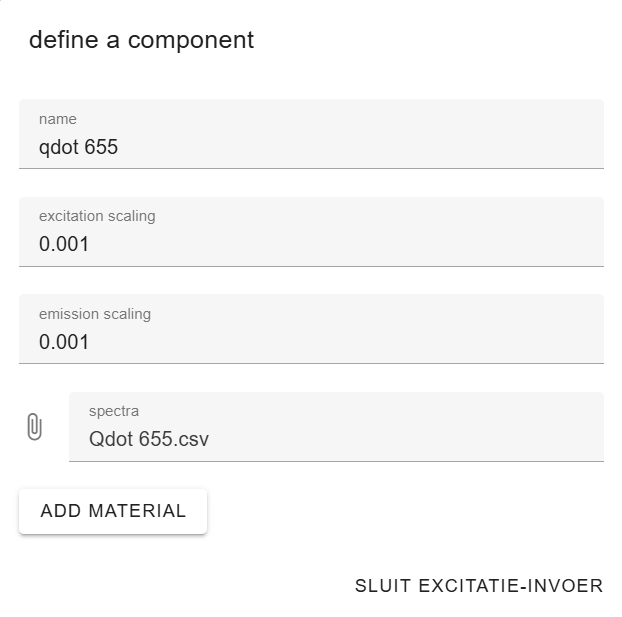
\includegraphics[width=0.5\linewidth]{custom_input_definition.png}
    \caption{Voorbeeld upload luminescent materiaal}%
    \label{fig:luminescent_input_definition}    
\end{figure}

De naam van het materiaal wordt gebruikt om alle nodige informatie van het materiaal op te slaan in een store voor de toegevoegde materialen. De data wordt opgeslagen in een object waarbij de keys de naam van het materiaal zijn en de values een object bevatten voor de excitatie- en emissiespectra. Daarnaast worden ook schalingswaarden opgeslagen. Deze schalingswaarden worden voorzien omdat we niet kunnen voorspellen hoe de waarden van de gebruiker zullen zijn. De schalingswaarden zorgen ervoor dat de gebruiker de data kan aanpassen zodat realistische waarden bekomen worden in de simulaties.

We kunnen de gebruiker van deze inputs een stuk minder laten aanpassen omdat bepaalde zaken zoals de golflengtes inherent zijn aan het materiaal. We laten de gebruiker wel nog toe om de volgende parameters aan te passen.

\begin{itemize}
    \item Schalingsfactoren
    \item concentratie
    \item \gls{plqy}
\end{itemize}

Omdat deze elementen ook geselecteerd moeten kunnen worden, hebben we componenten gemaakt die op basis van de geselecteerde waarde informatie ophalen uit de store en tonen aan de gebruiker. Hierbij moeten we rekening houden met de mogelijkheid dat de gebruiker een materiaal selecteert dat niet bestaat. In dat geval mag het component niet getoond worden. Dit kan eenvoudig gecontroleerd worden door te verifi\"eren of de naam behoort tot de beschikbare items en niet gelijk is aan LED, fosfor of QD.

\begin{figure}[H]
    \centering
    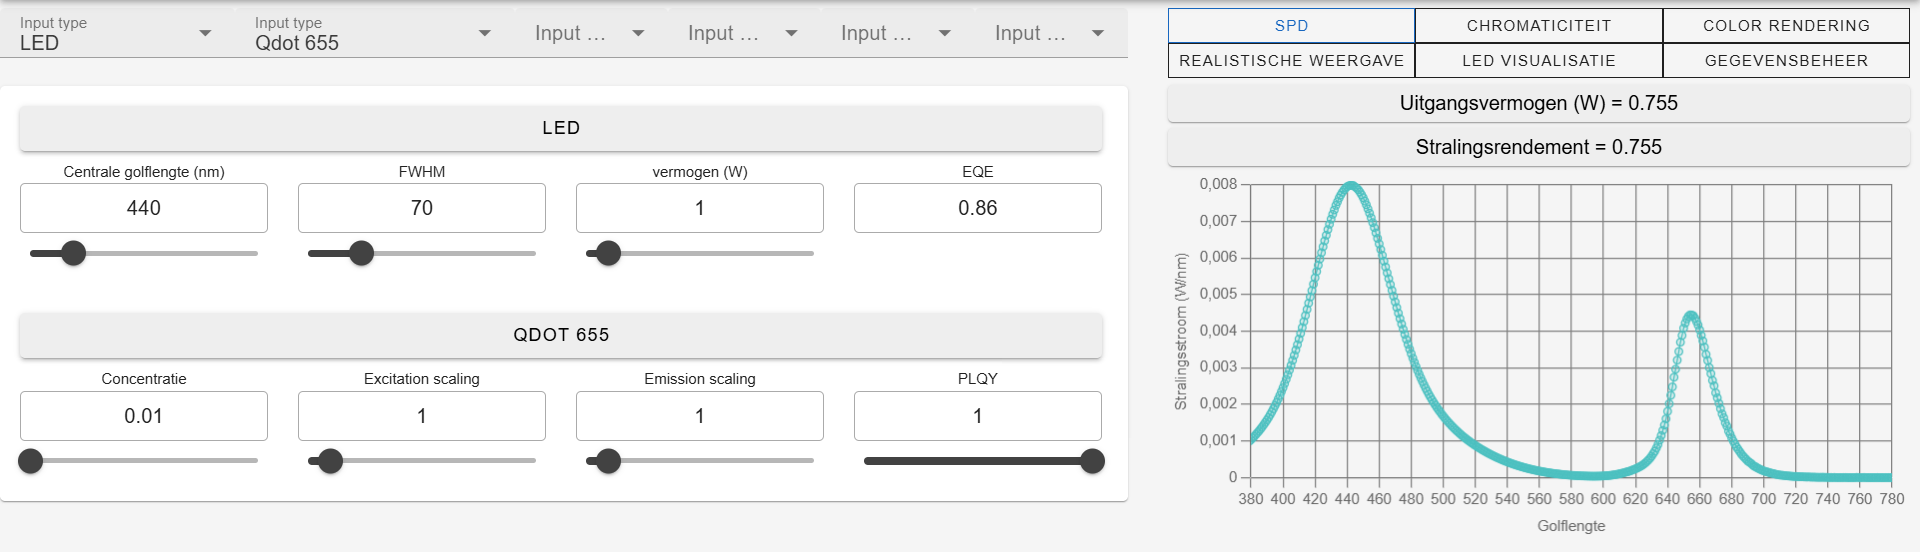
\includegraphics[width=1\linewidth]{qdot655_input.png}
    \caption{Voorbeeld luminescent materiaal input}%
    \label{fig:luminescent_input}
\end{figure}

\section{Implementatie LEDs en SPD}

\subsection{Implementatie LED model}

Het belangrijkste onderdeeel van de app dat we implementeerden, is het model van de \gls{led} en de omzetting ervan naar de \gls{spd}. We starten met een model of spectrum dat het relatieve vermogen per golflengte weergeeft. Op basis hiervan zetten we dit om naar de \gls{spd} van de \gls{led}.

Oorspronkelijk gebruikten we een gaussiaans model met het centrum op de centrale golflengte van de \gls{led} en een breedte bepaald door het \gls{fwhm}. Er zijn echter meerdere manieren om een \gls{led} te modelleren. Zo zouden we bijvoorbeeld ook een lorentziaans model kunnen gebruiken. Beide van deze modellen zijn echter relatief eenvoudig en geven geen volledig accuraat beeld van een \gls{led}. 

Om de simulaties accurater te maken, schakelden we over naar een wiskundig model dat specifiek ontwikkeld werd voor multichip \gls{led}s~\cite{ohnoSpectralDesignConsiderations2005}. Dit model wordt, net als het gaussiaanse model, bepaald door de centrale golflengte en het \gls{fwhm} van de \gls{led}. Het model bepaald de \gls{spd} van de \gls{led} aan de hand van de volgende formule:

\begin{equation}
    S_{\text{LED}}(\lambda, \lambda_0, \Delta \lambda_{0.5}) = \frac{\displaystyle g(\lambda, \lambda_0, \Delta \lambda_{0.5}) + 2g^5(\lambda, \lambda_0, \Delta \lambda_{0.5})}{3},
\end{equation}

waarin g gelijk is aan

\begin{equation}
    g(\lambda, \lambda_0, \Delta \lambda_{0.5}) = \exp\left(-\left[\frac{\lambda - \lambda_0}{\Delta \lambda_{0.5}}\right]^2\right).
\end{equation}

met symbolen:
\begin{itemize}
    \item \(\lambda\): De golflengte parameter (nm).
    \item \(\lambda_0\): De central golflengte van de \gls{led} emissie, dus de golflengte waarop het relatief vermogen het hoogste is.
    \item \(\Delta \lambda_{0.5}\): De \gls{fwhm}, stelt de spectrale breedte van de \gls{led} voor.
\end{itemize}

Omdat dit model een relatief model is, waarbij de hoogste waarde 1 is en de laagste 0, passen we een normalisatie toe om verdere berekeningen correct te laten verlopen. We normaliseren eenvoudigweg door de som van alle datapunten als normalisatiefactor te gebruiken. Door vervolgens elk datapunt door deze factor te delen, bekomen we een model met een totaal standaard vermogen van \'e\'en Watt. Omdat deze factor verschilt afhankelijk van de ingestelde parameters moeten we dit telkens opnieuw berekenen. Dit zorgt voor een lichte vertraging, we kiezen ervoor toch dit model te belijven gebruiken omdat de verhoogde accuraatheid belangrijker is dan de kleine vertraging. Dankzij deze aanpassing kunnen we het vermogen van een \gls{led} eenvoudig instellen door te vermenigvuldigen met het ingestelde vermogen. Daarnaast kunnen we de \gls{eqe} op dezelfde manier direct vermenigvuldigen.

\begin{figure}[H]
    \centering
    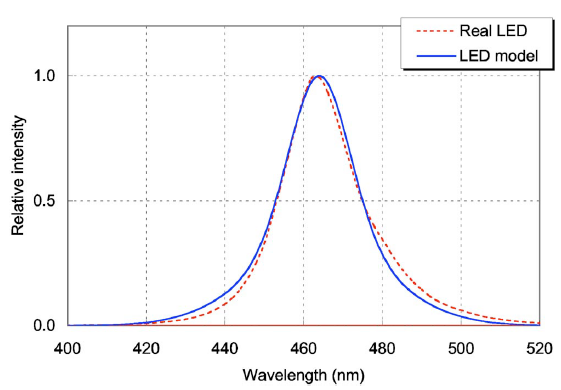
\includegraphics[width=0.8\linewidth]{figs/ohno.png}
    \caption{Multichip led model (Ohno)~\cite{ohnoSpectralDesignConsiderations2005}}%
    \label{fig:OhnoModel}
\end{figure}

\subsection{Implementatie SPD} % TO BE REWRITTEN

De overgang van een \gls{led}-model naar de \gls{spd} is vrij eenvoudig. Ten eerste maken we voor elke aanwezige \gls{led} de overgang van een relatief vermogen naar een effectief vermogen per nanometer. Door de eerder toegepaste normalisatie kunnen we dit doen door het relatieve vermogen van het model te vermenigvuldigen met het door de gebruiker ingestelde vermogen. Ten slotte vermenigvuldigen we ook de \gls{eqe} van de \gls{led}. Door deze vermenigvuldigingen krijgen we een realistische simulatie van de \gls{spd} van een \gls{led}. Wanneer een gebruiker meerdere \gls{led}s toevoegt, tellen we eenvoudigweg de verschillende bekomen \gls{spd}-waarden op om de totale \gls{spd} te verkrijgen.

Vervolgens tonen we het bekomen \gls{spd}-model aan de gebruiker in een grafiek. Hierin tonen we de stralingsstroom tussen 380 en 780 nm (het zichtbare spectrum). Naast deze grafiek geven we ook het uitgaande vermogen en de ''radiant efficiency'' (uitgaand vermogen / ingaand vermogen) weer. Dit helpt de gebruiker te begrijpen welke effecten verschillende technieken hebben op het genereren van witte \gls{led}s. Zo kan de gebruiker bijvoorbeeld zien waarom het combineren van rode, groene en blauwe \gls{led}s niet noodzakelijk even effici\"ent is als een blauwe \gls{led} met een gele fosfor.

Met deze grafiek kan de gebruiker zich al een eerste idee vormen over de eigenschappen van de gemaakte \gls{led}. Dit gebeurt aan de hand van de golflengtes van de pieken, de breedte van de pieken en de relatieve intensiteit van de pieken.

\subsection{Model EQE}\label{sec:eqe}

Omdat de berekening van de \gls{spd} gebruik maakt van de \gls{eqe} van een \gls{led}, is er ook een model voor nodig. Een realistisch model van \gls{eqe} is vooral belangrijk vanwege de ''green gap''. Dit is een kloof in de \gls{eqe}-waarden van \gls{led}s, die zich vooral bevindt bij de golflengtes die geassocieerd worden met groene \gls{led}s. Dit verklaart waarom het maken van witte \gls{led}s door simpelweg \gls{led}s te combineren momenteel ineffici\"ent is. Het \gls{eqe}-model leiden we af uit meetresultaten van \gls{led}s uit 2017 en 2018~\cite{hahnClosingGreenGapb}.  

Omdat het echter niet zeker is dat deze ''green gap'' blijft bestaan of even ernstig blijft, bieden we de gebruiker de mogelijkheid om een \gls{csv}-bestand met \gls{eqe}-waarden te uploaden. Dit bestand hoeft niet per se realistische waarden te bevatten. Zo kan het bijvoorbeeld ook worden gebruikt om te experimenteren met scenario's waarin de ''green gap'' niet bestaat of niet langer een groot probleem is. Dit maakt de app direct flexibeler en beter bestand tegen mogelijke veranderingen in de toekomst. Daarnaast laten we zo ook lerende gebruikers toe om te experimenteren met verschillende scenario's. Hierdoor kunnen ze beter begrijpen waarom de ''green gap'' een probleem is en hoe dit kan worden opgelost.

\begin{figure}[H]
    \centering
    \resizebox{0.7\textwidth}{!}{% This file was created with tikzplotlib v0.10.1.
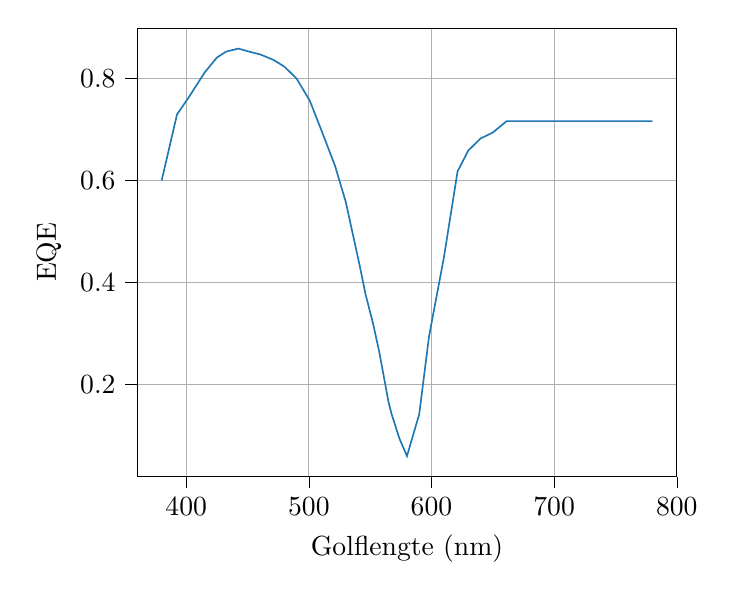
\begin{tikzpicture}

\definecolor{darkgray176}{RGB}{176,176,176}
\definecolor{steelblue31119180}{RGB}{31,119,180}

\begin{axis}[
tick align=outside,
tick pos=left,
x grid style={darkgray176},
xlabel={Golflengte (nm)},
xmajorgrids,
xmin=360, xmax=800,
xtick style={color=black},
y grid style={darkgray176},
ylabel={EQE},
ymajorgrids,
ymin=0.0188235315, ymax=0.8988234985,
ytick style={color=black}
]
\addplot [semithick, steelblue31119180]
table {%
380 0.6
392.5 0.7294
402.5 0.7647
415 0.81176
425 0.8411765
432.5 0.8529412
442.5 0.8588235
451.25 0.8529412
460.75 0.8470588
471.25 0.8364706
480 0.8235294
490 0.8
500.75 0.756706
510 0.7
521.25 0.6294118
530 0.5588235
541.25 0.4352941
546.25 0.3764706
552.5 0.3176471
557.5 0.2623529
565 0.1647059
567.5 0.1411765
573.75 0.09411765
580 0.05882353
590 0.1411765
598 0.2941176
610 0.4470588
621.25 0.6176471
630 0.6588235
640 0.6823529
650 0.6941176
661.25 0.716471
670 0.716471
780 0.716471
};
\end{axis}

\end{tikzpicture}
}
    \caption{Model \gls{eqe} ~\cite{hahnClosingGreenGapb}}
    \label{fig:eqe}
\end{figure}

\section{Implementatie chromaticiteit}

Voor het implementeren van de chromaticiteit maken we gebruik van de in \cref{sec:chromaticiteit} beschreven formules. Er moet echter een kleine aanpassing worden gemaakt. We moeten namelijk overgaan van integralen naar sommen. Dit omdat de \gls{spd} van een \gls{led} een discrete functie is (\'e\'en punt per nm). De chromaticiteit kan dan berekend worden aan de hand van de volgende formules voor de tristimuluswaarden:

\begin{align}
    X &= 683.\sum_{\lambda} \bar{x}(\lambda) S(\lambda) \Delta \lambda \\
    Y &= 683.\sum_{\lambda} \bar{y}(\lambda) S(\lambda) \Delta \lambda \\
    Z &= 683.\sum_{\lambda} \bar{z}(\lambda) S(\lambda) \Delta \lambda
\end{align}

waarin:

\begin{itemize}
    \item \(\bar{x}(\lambda)\), \(\bar{y}(\lambda)\) en \(\bar{z}(\lambda)\): de color matching functies.
    \item \(S(\lambda)\): de \gls{spd} van de \gls{led}.
    \item \(\Delta \lambda\): 1 nm.
\end{itemize}

De chromaticiteit kan dan berekend worden aan de hand van de volgende formules:

\begin{align}
    x &= \frac{X}{X + Y + Z} \\
    y &= \frac{Y}{X + Y + Z} \\
    z &= \frac{Z}{X + Y + Z}
\end{align}

Voor de berekening van de chromaticiteit maken we gebruik van de color matching functies. Om deze te gebruiken, laden we een \gls{csv}-bestand in met de waarden van de color matching functies (CIE 1931 2\textdegree observer). Deze waarden worden vervolgens gebruikt om de chromaticiteit te berekenen.

Om het berekende (x, y)-punt op het chromaticiteitsdiagram te tonen, gebruiken we een canvas-element (HTML element voor tekenen) met een foto van een standaard chromaticiteitsdiagram. We tekenen het punt op dit diagram door de (x, y)-co\"ordinaten te transformeren. Daarnaast voegen we de \gls{cct}-waarde toe, omdat het moeilijk voor de gebruiker is om deze waarde direct af te lezen van het diagram.

\begin{figure}[H]
    \centering
    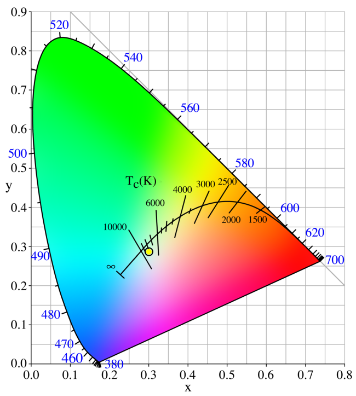
\includegraphics[width=0.5\linewidth]{figs/chromaticiteit_getekend.png}
    \caption{Voorbeeld resultaat chromaticiteit}%
    \label{fig:chromaticity_result}
\end{figure}

Het doel van de chromaticiteit is om de gebruiker een eerste idee te geven van de kleur van zijn gemaakte \gls{led}. Dit kan bijvoorbeeld de gebruiker helpen om een witte \gls{led} te maken. Daarnaast leert het de gebruiker ook dat chromaticiteit geen volledige beschrijving is van de kleur van een lichtbron. Zo kan een \gls{led} met dezelfde chromaticiteit toch een andere ervaring hebben voor een toeschouwer.

Naast de chromaticiteit worden ook de totale lichtstroom, het visueel rendement (totale lichtstroom / uitgaand vermogen) en de specifieke lichtstroom (totale lichtstroom / ingaand vermogen) getoond. De totale lichtstroom geeft de gebruiker een idee van het licht dat de \gls{led} uitstraalt. Het visueel rendement geeft de gebruiker inzicht in hoe effici\"ent de \gls{led} is in het omzetten van elektrische energie naar licht. De specifieke lichtstroom geeft de gebruiker een idee van hoeveel licht er wordt uitgestraald per watt elektrische energie. Deze waarden zijn belangrijk voor de gebruiker en kunnen bijvoorbeeld bepalend zijn bij het kiezen van een bepaalde manier om een kleur te verkrijgen (meerdere \gls{led} of luminescente materialen). Door ze hier toe te voegen krijgt de gebruiker dus een beter beeld van de eigenschappen van de gemaakte \gls{led}. Zo kan hij/zij bijvoorbeeld een \gls{led} maken met een bepaalde chromaticiteit, maar met een laag visueel rendement. Hierna kan dan bijvoorbeeld een \gls{led} bekomen worden met dezelfde chromaticiteit, maar met een hoger visueel rendement. Hierdoor leert de gebruiker over de voor en nadelen van de verschillende methoden om een kleur te bekomen.

\section{Implementatie color rendering}

\subsection{CIE Ra-15}

Het berekenen van de \gls{cri} en Ra-waarden is dankzij de Luxpy-bibliotheek zeer eenvoudig ~\cite{smetTutorialLuxPyPython2020}. De gebruiker hoeft enkel een \gls{spd} mee te geven, waarna de R0-R9-waarden berekend kunnen worden. Luxpy berekent automatisch het referentiespectrum, maar omdat we dit ook aan de gebruiker willen tonen, zodat deze kan proberen een (volgens \gls{cri}) zo goed mogelijke lichtbron te verkrijgen, hebben we de Luxpy-functie licht aangepast. Het referentiespectrum wordt door deze aaanpassing teruggegeven na een request aan de server. De \gls{cri}- en Ra-waarden worden vervolgens berekend en getoond aan de gebruiker in een staafdiagram.

We tonen de gebruiker de R0-R9-waarden, de \gls{cri}-waarde, het referentiespectrum en het eigen gemaakte spectrum. Aan de hand van de R-waarden kan de gebruiker zien welke kleuren goed worden weergegeven en welke niet. De \gls{cri}-waarde geeft de gebruiker een idee van hoe goed de kleuren over het algemeen worden weergegeven. Het referentiespectrum toont de gebruiker hoe een perfecte lichtbron eruitziet (volgens CIE Ra-15). We tonen al deze waarden zodat de gebruiker kan leren over de effecten van verschillende lichtbronnen op de kleurweergave.

Het is belangrijk dat de gebruiker leert hoe hij een lichtbron kan maken die volgens de \gls{cri}-waarde zo goed mogelijk is. Het is echter cruciaal dat de gebruiker begrijpt dat een hoge waarde niet noodzakelijk betekent dat de lichtbron effectief goed is. Zo kan bijvoorbeeld een score boven de 80 behaald worden, terwijl de waarde van R9 slechts rond de 20 ligt. Volgens \gls{cri} is dit een goede lichtbron, maar voor de mens is de R9-waarde erg belangrijk. In dit geval is de lichtbron waarschijnlijk niet ideaal. Hiervoor worden naast CIE Ra-15 ook andere methoden zoals IES TM-30 en ''realistic color rendering'' aangeboden.

\subsection{ies-tm30}

Naast CIE Ra-15 biedt Luxpy ~\cite{smetTutorialLuxPyPython2020} ook de mogelijkheid om IES TM-30-berekeningen uit te voeren en rapporten te genereren. Omdat dit een recentere en offici\"ele color rendering maat is, kozen we ervoor de gebruiker de mogelijkheid te geven om IES TM-30 te gebruiken in plaats van CIE Ra-15. Daarnaast is het ook een goede manier om te leren over de verschillen tussen verschillende maten voor kleurweergave. Een meer geavanceerde gebruiker kan dan weer kiezen welke color rendering methode het beste past bij zijn of haar toepassing. Net als bij CIE Ra-15 kunnen de benodigde berekeningen uitgevoerd worden met Luxpy.

We kozen ervoor om een eenvoudig TM-30-verslag te gebruiken met Rf, Rg, CCT en D(u,v), omdat dit de belangrijkste waarden binnen de TM-30 methode zijn. Daarnaast tonen we een gamutcirkel met daarop hue shift vectoren. Aan de hand van deze waarden kan een lerende gebruiker leren over het belang van de verschillende metrieken. Een geavanceerde gebruiker kan zich een idee vormen over de geschiktheid van zijn gemaakte lichtbron voor een bepaalde toepassing.

\section{Implementatie luminescente materialen}

Om de invloed van luminescente materialen te begrijpen, hebben we een berekening nodig die van de excitatie- en absorptiespectra naar de geabsorbeerde en ge\"emitteerde energie leidt. Zoals eerder vermeld, zijn er geen applicaties die dit reeds hebben gedaan. Bovendien zijn er geen formules beschikbaar die dit op een eenvoudige en algemene manier kunnen berekenen. Daarom besloten we zelf een formule te ontwikkelen.

\subsection{Simpele berekening}

oorspronkelijk maakten we gebruik van een simpele berekening die ook in de KU Leuven Excel werd gebruikt. Deze werkt echter alleen volledig correct voor fosforen. Daarnaast is deze niet volledig theoretisch onderbouwd, maar volgt deze de verwachte effecten van fosforen (zoals de Stokes shift). De geabsorbeerde energie wordt in deze methode berekend aan de hand van een exponentieel verval.

\begin{equation} E_{abs} = \text{S} . (1 - \exp(-\text{C}.3.\sqrt{2.\pi}.\text{norm}(\lambda,\lambda_{ex},\text{excitatiebreedte/2}) )) \end{equation} waarbij C de concentratie is en S de stralingsstroom.\

Omdat deze formule gebaseerd is op het gebruik van de normale verdeling binnen het exponenti\"ele verval, is deze alleen correct voor fosforen. Voor quantum dots en andere materialen waarbij de excitatiespectra geen normale verdeling volgen, is deze formule minder geschikt.

Om het ge\"emitteerde vermogen te berekenen, maken we gebruik van een simpele formule waarin we rekening houden met de verschillen in concentraties tussen de verschillende aanwezige materialen en de Stokes shift.

\begin{equation} E_{em} = E_{abs} . QE . \text{emissiespectrum} . C . (1 - (\lambda_{em}-\lambda_{ex}/\lambda_{ex})) \end{equation} waarbij C het percentage van alle luminescente materialen is dat deze inneemt.

%figure
\begin{figure}[H]
    \centering
    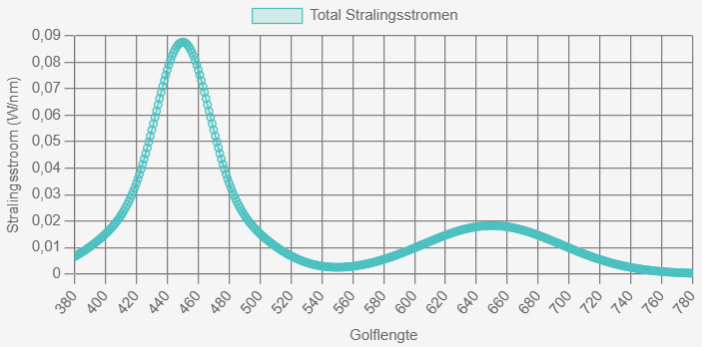
\includegraphics[width=0.45\linewidth]{figs/spectrum_fosfor_simple.png}
    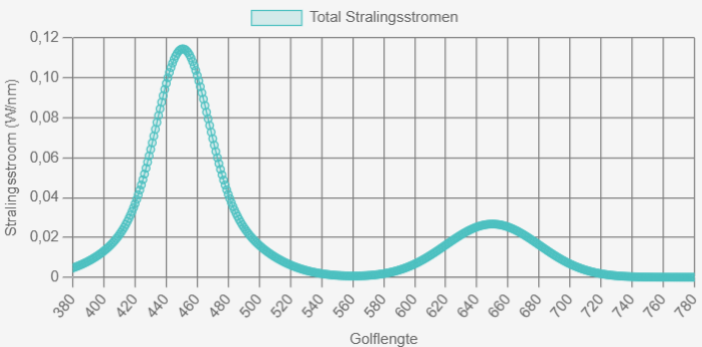
\includegraphics[width=0.45\linewidth]{spectrum_QD_simple.png}
    \caption{Voorbeeld resultaten met simpel model (links = fosfor, rechts = quantum dot)}%
    \label{fig:result_simple}
\end{figure}

\subsection{Geavanceerde berekening}\label{sec:advanced}

Om een correctere berekening te maken zodat een lerende gebruiker de effecten van luminescente materialen correct kan leren kennen ontwikkelden we een geavanceerd model. We ontwikkelden dit geavanceerd model op een meer theorethische manier zodat alle effecten van de luminescente materialen correct gemodeleerd zijn.
Deze formule baseren we op de verdeling van fotonen en de verdeling van energie.
Daarnaast maken we gebruik van de relaties tussen excitatie- en emissiespectra en de
geabsorbeerde en ge\"emiteerde energie.
Deze formule kan gebruikt worden voor elk luminescent materiaal waarvan de
excitatie- en emissiespectra gekend zijn en is dus meer geschikt voor de toepassing dan de simpele formule.

We weten dat 

\begin{equation}
    f_1(\lambda) = \text{De distributie van geabsorbeerde energie en}
\end{equation}
\begin{equation}
    f_2(\lambda) = \text{De distributie van ge\"emiteerde energie}.
\end{equation}

Hierbij weten we dat 

\begin{equation}
    f_1(\lambda) = f'_1(\lambda) . SPD(\lambda)
\end{equation}
met $f'_1(\lambda)$ het excitatiespectrum van het gebruikte luminescente materiaal.

Nu moet echter nog $f_2(\lambda)$ berekend worden. We weten dat de distributie van het aantal fotonen evenredig is met

\begin{equation}
    f(\lambda).\lambda = g(\lambda) \text{ (de verdeling van de fotonen)} \label{eq:distFot}
\end{equation}
want
\begin{equation}
    E(\lambda) \sim 1/\lambda \text{ (de energie van een foton)}
\end{equation}

Als we veronderstellen dat \gls{plqy} = 100\% (het aantal geabsorbeerde fotonen/het aantal ge\"emiteerde fotonen van een materiaal). Dan weten we dat het aantal fotonen gelijk blijft en kunnen we stellen dat

\begin{equation}
    \int g_1(\lambda) \, d\lambda = \int g_2(\lambda) \, d\lambda
\end{equation}
Met $g(\lambda)$ de verdeling van de fotonen.

uit \ref{eq:distFot} volgt dan dat

\begin{equation}
    \int f_1(\lambda).\lambda \, d\lambda = \int f_2(\lambda).\lambda \, d\lambda
\end{equation}
Met 

Omdat $f_1(\lambda)$ gekend is en we de vorm van $f_2(\lambda)$ kennen. Deze heeft namelijk dezelfde vorm als het emissiespectrum $f'_2(\lambda)$. We kennen dus $f_2(\lambda)$ op een schalingsfactor na dus

\begin{equation}
    f_2(\lambda) = a.f'_2(\lambda)
\end{equation}
Met $f'_2(\lambda)$ het emissiespectrum van het luminescente materiaal en a de schalingsfactor.

Dan kunnen we a op de volgende manier vinden

\begin{equation}
    \int f_1(\lambda).\lambda \, d\lambda = \int a.f'_2(\lambda).\lambda \, d\lambda
\end{equation}

\begin{equation}
    \Leftrightarrow
    a = \int f_1(\lambda).\lambda \, d\lambda / \int f'_2(\lambda).\lambda \, d\lambda
\end{equation}

Tot nu toe hebben we verondersteld dat \gls{plqy} gelijk is aan 100\%. Dit zal echter meestal niet het geval zijn. Om hier rekening mee te houden vermenigvuldigen we op het einde nog met \gls{plqy} en is dus

\begin{equation}
    f_2(\lambda) = a.PLQY.f'_2(\lambda)
\end{equation}

\begin{figure}[H]
    \centering
    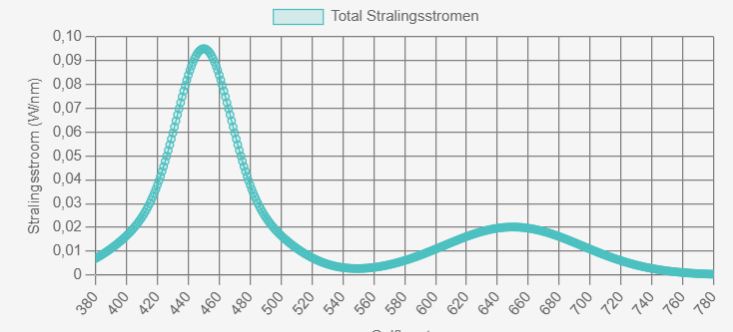
\includegraphics[width=0.45\linewidth]{spectrum_fosfor_advanced.png}
    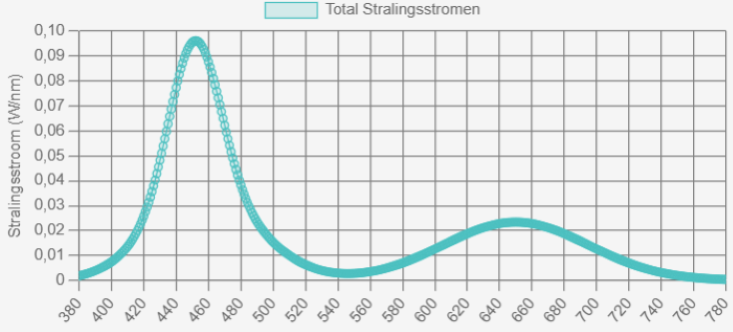
\includegraphics[width=0.45\linewidth]{spectrum_QD_advanced.png}
    \caption{Voorbeeld resultaten met geavanceerd model (links = fosfor, rechts = quantum dot)}%
    \label{fig:result_advancded}
\end{figure}

Zoals te zien is in \ref{fig:result_simple} en \ref{fig:result_advancded} 
zijn de resultaten bij het gebruik van fosforen inderdaad zeer vergelijkbaar.
Bij quantum dots is er echter een groot verschil. 
Dit omdat nu correct rekening gehouden wordt met de niet normale verdeling van
het excitatiespectrum.

\subsection{Spectra}

We maken gebruik van een algemeen model van de spectra zodat we de gebruiker kunnen laten zien wat de effecten zijn van de verschillende
parameters van luminescente materialen. Hiervoor moeten we dus per standaard materiaal een model gemaakt worden.

Voor fosforen maakten we een model dat een normale verdeling volgt. Dit omdat de meeste
fosforen een excitatie- en emissiespectrum hebben die ongeveer een normale verdeling volgen. Deze
zijn meestal beiden gecentreerd rond de excitatie- en emissiegolflengte met een bepaalde
''skew''. Het is dan ook voor deze reden dat we de mogelijkheid voorzien om het model aan te passen naar bijvoorbeeld een normaalverdeling met ''skew'' (\cref{sec:data_manager}).

\begin{figure}[H]
    \centering
    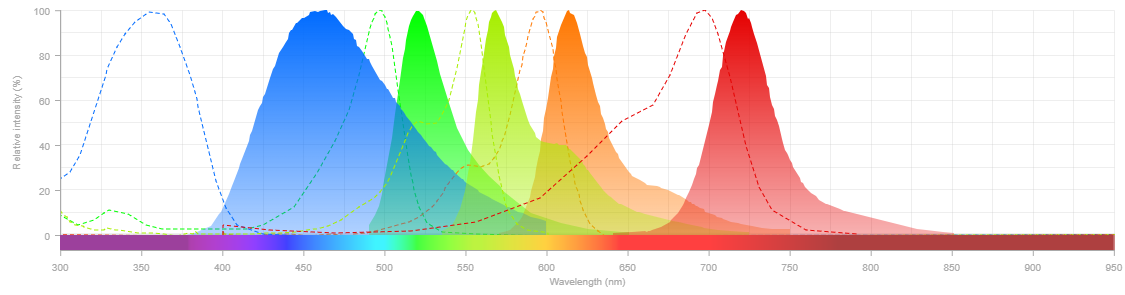
\includegraphics[width=0.9\linewidth]{spectraviewer_normPhos.png}
    \caption{Voorbeeld fosfor spectra (stippellijn = excitatie, vol = emissie) ~\cite{FluorescenceSpectraViewer}}%
    \label{fig:spectra_fosfor}
\end{figure}

Het modeleren van quantum dots is echter moeilijker. Ze hebben net zoals
fosforen een normaal verdeeld emissiespectrum. Het excitatiespectrum is echter
niet normaal verdeeld. Ze volgen eerder een dalende lijn.

\begin{figure}[H]
    \centering
    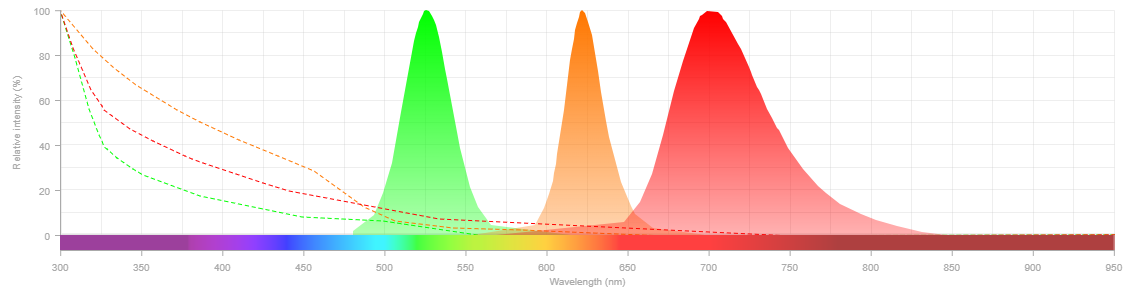
\includegraphics[width=0.9\linewidth]{spectraviewer_QD.png}
    \caption{Voorbeeld fosfor QD (stippellijn = excitatie, vol = emissie) ~\cite{FluorescenceSpectraViewer}}%
    \label{fig:spectra_QD}
\end{figure}

Daarnaast zijn er ook in de lijn soms pieken te zien. Ten laatste varieert de lijn ook sterk afhankelijk van de configuratie van de quantum dot. Dit maakt het modelleren van quantum dots moeilijker dan fosforen. Zo bestaan er wel modellen voor quantum dots maar
zijn deze vaak zeer specifiek afhankelijk van de configuratie van de quantum dot. Dit zijn dan bijvoorbeeld modellen die een empirische fit zijn van meetresultaten.

Omdat we een zo algemeen mogelijk model willen maken voor het excitatiespectrum is dit type model dus geen goede optie. Ook zou het aanpassen van dit type
model weinig bruikbaar zijn omdat het meestal gebruik maakt van moeilijkere parameters. Die ook weinig relevant zijn voor de gebruiker van onze app.

Uit deze vaststellingen besloten we om een simpel model te gebruiken voor het excitatiespectrum
van de quantum dots. Dit model volgt een dalende exponentiele lijn. Dit model is echter niet
perfect en dus voorzien we de optie om de gebruikte formule aan te passen. Daarnaast voorzien we hiervoor ook de mogelijkheid om eigen luminescente materialen toe te voegen. Dit bijvoorbeeld met gemeten data van een specifieke quantum dot voor volledige accuraatheid.

\begin{equation}
    0.03 . \exp\left(\frac{\log(0.1) . (\lambda - 360)}{\lambda_{em} - 360}\right)
\end{equation}

\begin{figure}[H]
    \centering
    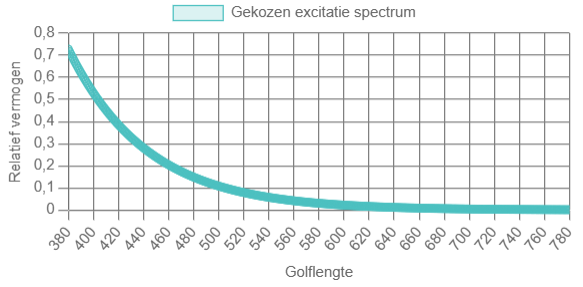
\includegraphics[width=0.9\linewidth]{excitatie_QD.png}
    \caption{Standaard excitatiespectrum qunatum dot}%
    \label{fig:basic_ex_QD}
\end{figure}

\section{Implementatie LED visualisatie}

De led visualisatie wordt ge\"implementeerd aan de hand van Konva. Dit is een library die het eenvoudig maakt om op een canvas te tekenen. Ze zorgt ervoor dat we makkelijk mooiere figuren kunnen maken worden dan met de standaard canvas van HTML. Daarnaast is het ook eenvoudig om interactie aan de figuur toe te voegen. Dit omdat we kunnen gebruik maken van Konva voor Vue. Dit is een library die het eenvoudig maakt om Konva te gebruiken in combinatie met Vue en dus reactiviteit aan Konva toevoegt.

De visualisatie is vrij simpel (\cref{fig:led_vis}), ze bestaat uit een trapezium met hierin rechthoeken, punten en kristallen. De trapezium stelt de chip voor, de rechthoeken de \gls{led}s, de kristallen de fosforen en de punten de quantum dots.

De ingestelde waarden van de gebruiker hebben invloed op de gemaakte figuur. Zo bepaald de golflengte/emissiegolflengte de kleur van de objecten in de chip. De concentratie van de luminescente materialen bepaald dan weer de hoeveelheid van deze materialen in de chip.

Om de kleur van de objecten te bepalen maken we gebruik van een eenvoudige berekening om de golflengte om te zetten naar een hexadecimale kleurwaarde. De berkening werkt binnen bepaalde bereiken van golflengtes en zet hierin telkens de rode, groene en blauwe waarde. In het bereik tussen 380 en 440nm wordt bijvoorbeeld blauw op \'e\'en gezet, groen op 0 en rood krijgt een waarde afhankelijk van de volgende formule:

\begin{equation}
    \text{rood} = -(\lambda - 440) / (440 - 380)
\end{equation}

Ten slotte wordt nog een factor en een gamma toegevoegd. De factor zorgt ervoor dat de intensiteit minder sterk wordt wanneer de grenzen van het zichtbare licht bereikt worden. Het gamma zorgt ervoor dat de kleuren er natuurlijker uitzien. Dit gamma wordt op 0.8 geplaatst. Door voor rood, groen en blauw de volgende berekening uit te voeren bekomen we de uiteindelijke kleurwaarde:

\begin{equation}
    \text{kleur} = \begin{cases}
        255 \cdot (\text{waarde}\cdot\text{factor})^{\text{gamma}} & \text{als waarde} > 0 \\
        0 & \text{anders}
    \end{cases}
\end{equation}

We implementeren de visualisatie op deze manier om de gebruiker een eenvoudig beeld te geven over hoe een door hem gemaakte \gls{led} eruit zou zien. Dit kan de gebruiker helpen begrijpen hoe een chip ongeveer is opgebouwd en hoe de verschillende materialen in de chip zouden kunnen geplaatst zijn op een eenvoudige wijze.

\begin{figure}[H]
    \centering
    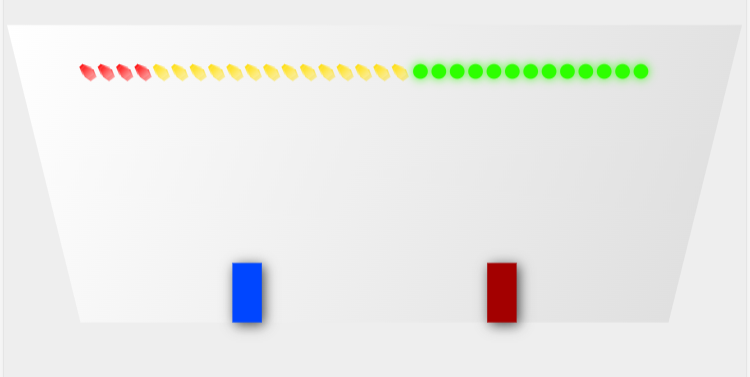
\includegraphics[width=0.9\linewidth]{led_vis.png}
    \caption{Voorbeeld LED visualisatie (2 fosforen, 1 QD en 2 LEDs)}%
    \label{fig:led_vis}
\end{figure}

\section{Implementatie hyperspectral image rendering}

Voor hyperspectral image rendering gebruiken we net zoals voor color rendering de luxpy bibliotheek ~\cite{smetTutorialLuxPyPython2020}. Als we echter gewoon de standaard implementatie gebruiken zorgt het in dit geval voor problemen. Dit omdat het uitvoeren van de standaardimplementatie op de server maar liefst 15 minuten duurt. Daarnaast gebruikt deze methode ook een grote hoeveelheid geheugen. Als dus
meerdere mensen tegelijk deze standaardimplementatie zouden gebruiken zou de server al rap niet genoeg geheugen hebben en crashen. Daarnaast vinden we 15 minuten zeker een stuk te lang voor een gebruiker om te wachten op het resultaat van de rendering. 

Om dit probleem op te lossen onderzochten we twee mogelijke oplossingen:
\begin{itemize}
    \item Aanpassen van de gebruikte foto.
    \item Berekeningen die niet veranderen opslaan.
\end{itemize} 

\subsection{Foto}

De standaard foto \ref{fig:std_img_luxpy} die luxpy ~\cite{smetTutorialLuxPyPython2020} gebruikt is een vrij complexe foto met een hoge
resolutie. Deze combinatie van de hoge resolutie en de vele kleueren in de foto
zorgt ervoor dat de berekeningen langer duren dan gewenst. Om dit op te lossen keken we naar twee oplossingen:

\begin{itemize}
    \item Resolutie verlagen
    \item Complexiteit foto verlagen
\end{itemize}

\begin{figure}[H]
    \centering
    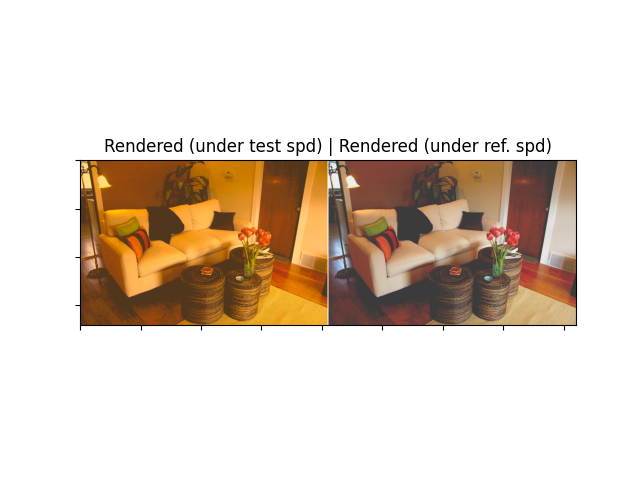
\includegraphics[width=0.8\linewidth]{standard_image.png}
    \caption{Standaard foto luxpy ~\cite{smetTutorialLuxPyPython2020}}%
    \label{fig:std_img_luxpy}
\end{figure}

Ten eerste onderzochten we het gebruik van een simpelere foto. We gebruikten hiervoor eerst een heel simpele foto van een blauwe bal \ref{fig:blue_ball} op een witte achtergrond. Dit verbeterde de snelheid van de berekening sterk, maar bracht een belangrijk probleem met zich mee: de foto geeft weinig informatie over de belichting.

Het grootste probleem is namelijk dat een gebruiker niet kan weten hoe de bal er normaal uitziet. Er bestaan namelijk zeer veel blauwe ballen in zeer veel verschillende tinten blauw. Het is dus hierdoor ook moeilijk af te leiden wat het effect van de gebruikte belichting is. De gebruiker kan dus niet leren over de effecten van de belichting op de kleur van het object.

\begin{figure}[H]
    \centering
    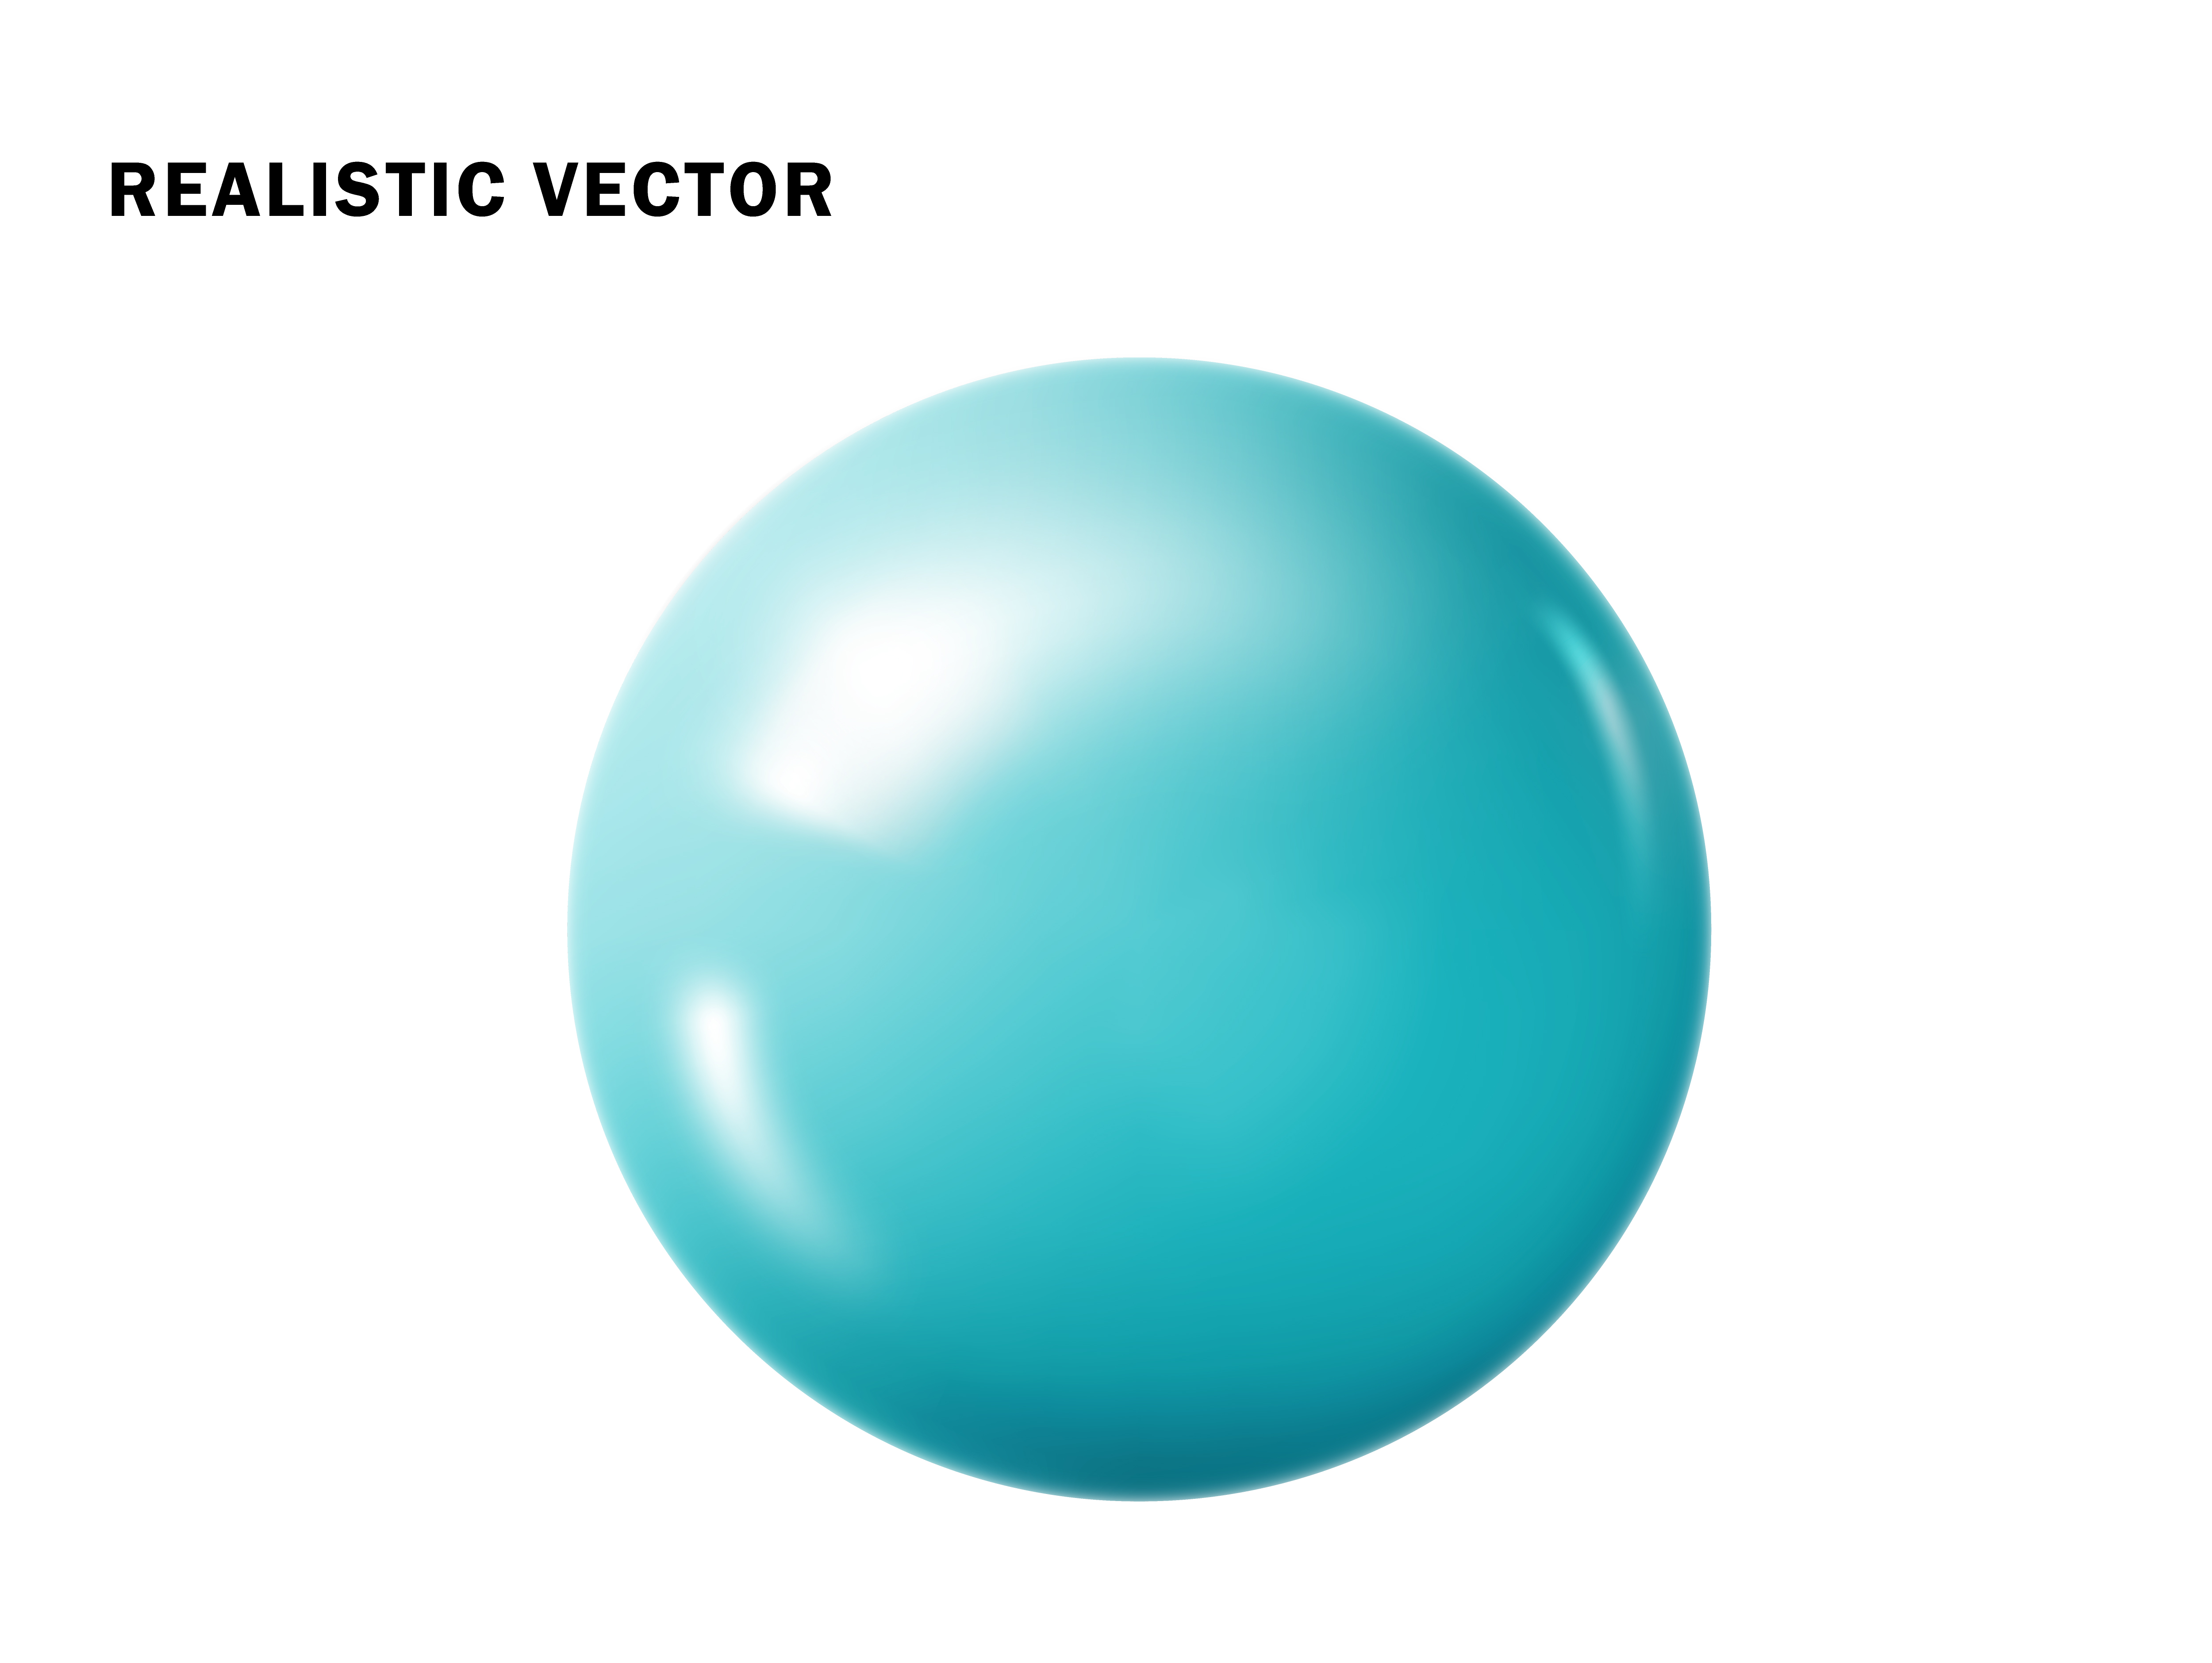
\includegraphics[width=0.4\linewidth]{blue_ball_copyright.jpg}
    \caption{Foto blauwe bal}%
    \label{fig:blue_ball}
\end{figure}

Om dit op te lossen keken we naar een eenvoudigere foto, die echter wel voorwerpen bevat waarvan de gebruiker de kleur zeker kent. Zo kwamen we op het idee om een verzameling fruit op een witte achtergrond te gebruiken, zoals te zien is in Figuur \ref{fig:fruit}.

Hierdoor blijft de hoeveelheid kleuren beperkt en hebben waardoor de versnelling optreed. Daarnaast hebben de meeste voorwerpen een vaste kleur wat ervoor zorgt dat de gebruiker de normale kleur van de voorwerpen kent. Deze verbetering zorgde echter nog niet voor genoeg winst in snelheid, dus onderzochten we ook de resolutie.

\begin{figure}[H]
    \centering
    \includegraphics[width=0.6\linewidth]{fruit_nocopyright.jpg}
    \caption{Foto fruit 6,99MB}%
    \label{fig:fruit}
\end{figure}

Ten tweede keken we naar de resolutie van de foto. Dit betekende simpelweg dat we de foto verkleinden. We deden dit systematisch totdat we een versie kregen die zowel een voldoende snelle berekening als een scherp genoeg beeld opleverde. Uiteindelijk verkleinden we de foto van 6,99 MB naar 9,09 kB, zoals te zien is in Figuur \ref{fig:fruit_small}. Het is mogelijk de foto nog verder te verkleinen, maar dit zou ten koste gaan van de kwaliteit van de foto. We vonden dat de kwaliteit van de foto in Figuur \ref{fig:fruit} nog voldoende was om de gebruiker een goed beeld te geven van de belichting van de foto. Bij kleinere foto's beginnen bepaalde details verloren te gaan, wat het moeilijker maakt voor de gebruiker om de belichting correct in te schatten.

\begin{figure}[H]
    \centering
    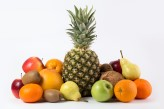
\includegraphics[width=0.6\linewidth]{fruit_nocopyright_3.jpg}
    \caption{Foto fruit 9,09kB}%
    \label{fig:fruit_small}
\end{figure}

Met een combinatie van deze twee aanpassingen op de foto bekomen we een foto die snel genoeg is ($\pm$ 5 seconden) om te renderen en toch voldoende informatie bevat voor de gebruiker.

\subsection{Berekeningen}

Om de berekening nog sneller te maken keken we ook naar het opslaan van niet veranderende berekeningen. Zo zal de rendering van de verschillende beschikbare referentiespectra bijvoorbeeld nooit veranderen. We kunnen de rendering van de referentiespectra dus opslaan en deze opnieuw gebruiken bij elke berekening van de rendering.

Deze aanpassing zorgt ervoor dat de rendering zelf een stuk sneller kan verlopen doordat, maar half zo veel werk moet gebeuren. Doordat we echter reeds de tijd van de berekening sterk verlaagt hebben door de aanpassingen aan de foto, is het effect van deze aanpassing minder groot. Doordat de resolutie voor een grote verandering in tijd zorgt, treed er een probleem op bij het voordien berekenen van de foto. Door de lage resolutie is namelijk de tijd die nodig is voor het berekenen van het referentiespectra gedeelte ongeveer gelijk aan de tijd die nodig is voor het inladen van de foto. Hierdoor is het effect van het voordien berekenen van het referentiespectra verwaarloosbaar. Moesten we echter in de toekomst een foto met een grotere resolutie willen gebruiken kan deze aanpassing mogelijks wel een voldoende groot effect hebben.

\section{Implementatie data manager}\label{sec:data_manager}

We maken de app bruikbaarder voor geavanceerde gebruikers door een data manager toe te voegen. Hierin krijgt de gebruiker de mogelijkheid om gebruikte defaults aan te passen en te bekijken. Daarnaast kan de gebruiker eigen luminescente materialen toevoegen.

De eerste functie in de data manager is het vergrendelen van bepaalde variabelen. Met deze functionaliteit kan de gebruiker verschillende parameters van de inputs vergrendelen of ontgrendelen. Dit is vooral bedoeld voor educatieve doeleinden, bijvoorbeeld wanneer een docent leerlingen vraagt om een specifieke waarde, zoals de excitatiebreedte, vast in te stellen.

Daarnaast kan de gebruiker het referentiespectrum voor de realistic rendering aanpassen. Hierbij kan hij kiezen uit standaard spectra zoals D65, Tungsten, Clear Sky en Daylight. Voor color rendering kan hij bovendien het CRI-type instellen (CIE Ra-15, IES TM-30).

Ten derde kan de gebruiker de formules voor de standaard spectra van luminescente materialen en het LED-emissiemodel aanpassen. Hij kan gebruikmaken van standaard formules en parameters om een wiskundige formule te defini\"eren voor de spectra van de luminescente materialen. Deze formule kan vervolgens worden in- of uitgeschakeld. Tijdens het maken van de formule tonen we een grafiek van het gegenereerde spectrum om het beslissingsproces te vergemakkelijken.

\begin{figure}[H]
    \centering
    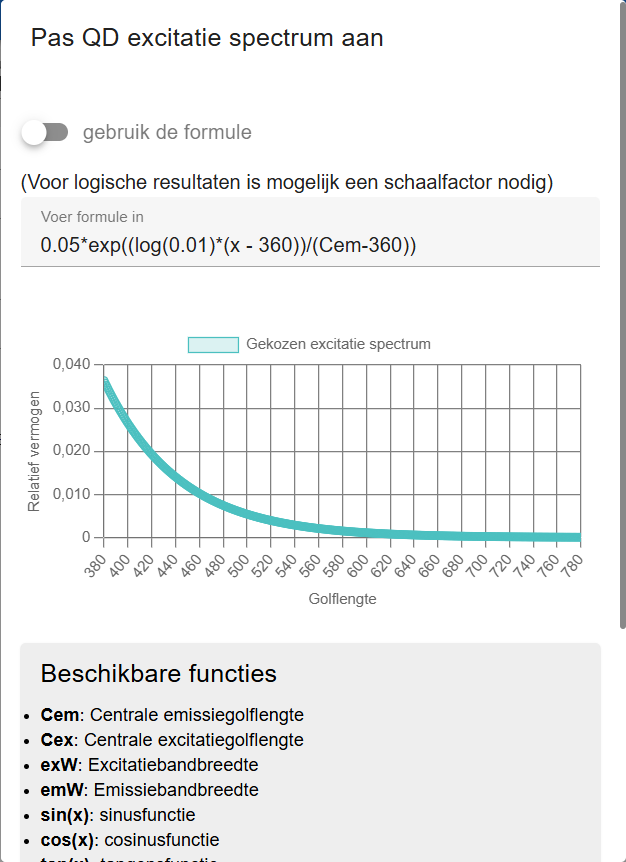
\includegraphics[width=0.5\linewidth]{Formula_input.png}
    \caption{Voorbeeld input formule}%
    \label{fig:formula_input}
\end{figure}

Ten vierde krijgt de gebruiker in de data manager inzicht in de verschillende gebruikte standaardparameters. Zo kan hij de standaard EQE-waarden, het standaard LED-emissiemodel en de eigenschappen van luminescente materialen bekijken. Daarnaast tonen we bij de EQE- en LED-emissiemodeldata ook de bron van deze gegevens.

Zoals eerder vermeld, kan de gebruiker ook eigen luminescente materialen toevoegen \ref{sec:luminescent_input}. Tot slot kan hij de gebruikte \gls{eqe}-waarden aanpassen. Dit gebeurt via een \gls{csv}-bestand, zoals beschreven in \ref{sec:eqe}.

\section{Hosting}

De webapp wordt gehost op een combinatie van nginx (frontend) en systemctl (Flask-backend). Nginx fungeert niet alleen als host voor de frontend, maar ook als reverse proxy. Hierdoor kan het de requests van de frontend naar de backend sturen en tegelijkertijd rate limiting toepassen. Dit voorkomt overbelasting van de server, vooral bij rekenintensieve processen zoals hyperspectral image rendering, die veel tijd in beslag nemen.